%% algorithm.tex — Solution Methodology
%% Many-to-Many DRT Bidirectional Meeting Point Paper
%% Section 6 of the paper.

% ============================================================
\section{Solution Methodology}\label{sec:algorithm}
% ============================================================

The problem defined in Section~\ref{sec:model} is NP-hard (see
Section~\ref{subsec:complexity}). We develop two complementary solution approaches: an
exact MILP formulation solved by Gurobi for small instances, and a rolling horizon
Adaptive Large Neighborhood Search (ALNS) heuristic for real-time operation at scale.

% ------------------------------------------------------------
\subsection{Exact Algorithm: MILP Formulation}\label{subsec:milp}
% ------------------------------------------------------------

For small instances, we formulate the static batch version of the problem as a
Mixed-Integer Linear Program (MILP) to obtain provably optimal solutions. These serve as
benchmarks for validating heuristic quality.

\paragraph{Decision Variables.}
The MILP uses binary assignment variables $x_{r,m^P,m^D,v} \in \{0,1\}$, equal to 1 if
request $r$ is assigned to meeting point pair $(m^P, m^D) \in M_r^P \times M_r^D$ and
served by vehicle $v \in \mathcal{V}$. Continuous variables $s_{v,i} \geq 0$ represent
the scheduled service time at node $i$ in vehicle $v$'s route. The acceptance indicator
is recovered as $z_r = \sum_{m^P, m^D, v} x_{r,m^P,m^D,v}$.

\paragraph{Objective.}
The MILP minimizes the same weighted cost (Equation~\ref{eq:objective}), with each cost
component linearized in terms of $x_{r,m^P,m^D,v}$ and $s_{v,i}$.

\paragraph{Constraints.}
The formulation enforces all fourteen operational constraints
(\ref{con:capacity})--(\ref{con:domain-md}). Capacity constraint~(\ref{con:capacity}) is
linearized using standard load-tracking variables. Time-window
constraints~(\ref{con:tw-early})--(\ref{con:tw-late}), ride-time
constraint~(\ref{con:ridetime}), and route time consistency~(\ref{con:time-consistency})
are expressed as linear inequalities in $s_{v,i}$. Walking radius
constraints~(\ref{con:walk-pickup})--(\ref{con:walk-dropoff}) are enforced implicitly by
restricting the domain of $x_{r,m^P,m^D,v}$ to feasible meeting point pairs.

\paragraph{Solver and Scope.}
The MILP is solved using Gurobi~10. Instances with up to 30--50 passengers and 5--8
vehicles are tractable within a 300-second time limit; Gurobi reports the optimality gap
for instances where the time limit binds. The MILP is not intended for real-time use; its
role is to provide exact benchmarks on small instances for validating the heuristic.

\begin{figure}[h]
\centering
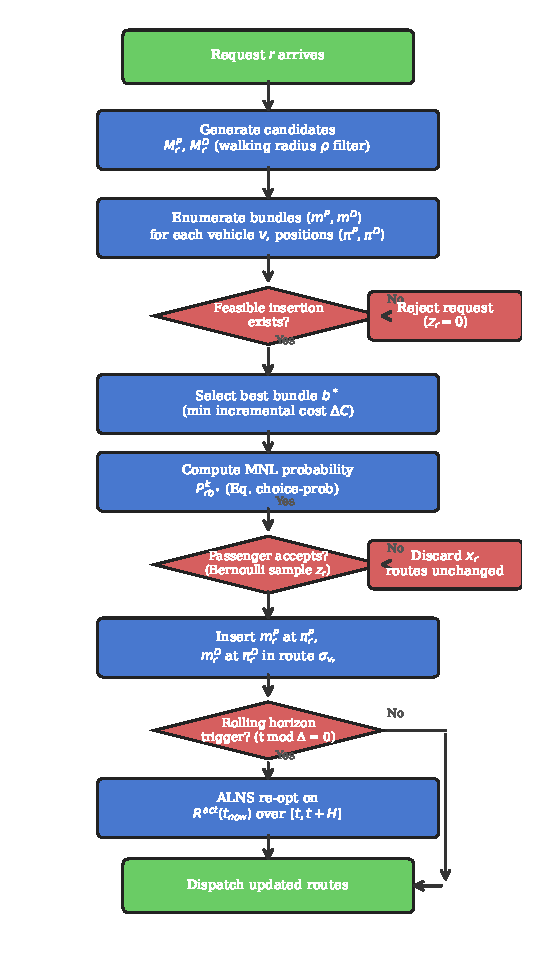
\includegraphics[width=\columnwidth]{../figures/fig03_algorithm}
\caption{Online insertion and rolling horizon ALNS algorithm flowchart.}
\label{fig:algorithm}
\end{figure}

% ------------------------------------------------------------
\subsection{Heuristic Algorithm: Rolling Horizon ALNS}\label{subsec:alns}
% ------------------------------------------------------------

For real-time operation, we develop a rolling horizon ALNS heuristic that processes
arriving requests online and periodically re-optimizes committed routes. The algorithm
follows the three-layer architecture of Section~\ref{sec:three-layer}.

\subsubsection{Candidate Generation}

Upon arrival of request $r$, the system generates candidate meeting point sets $M_r^P$
and $M_r^D$ by filtering $\mathcal{M}$ against walking radii $\rho^P$ and $\rho^D$
(constraints~\ref{con:walk-pickup}--\ref{con:walk-dropoff}), then retaining the
top-$k^{\text{top}}$ candidates ranked by proximity to $o_r$ and $\delta_r$ respectively.
This yields $|M_r^P| \leq k^{\text{top}}$ pickup candidates and
$|M_r^D| \leq k^{\text{top}}$ dropoff candidates. The filtering step runs in
$O(|\mathcal{M}| \log |\mathcal{M}|)$ per request using a pre-sorted distance index.

\subsubsection{Online Insertion Evaluation}

For each bundle $(m^P, m^D) \in M_r^P \times M_r^D$, the algorithm enumerates all
vehicles $v \in \mathcal{V}$ and all insertion position pairs $(\pi^P, \pi^D)$ with
$\pi^D > \pi^P$ (constraint~\ref{con:precedence-pos}). Feasibility against
constraints~(\ref{con:capacity}), (\ref{con:tw-early})--(\ref{con:tw-late}),
(\ref{con:ridetime}), and (\ref{con:time-consistency}) is checked in $O(1)$ per position
pair using forward and backward schedule arrays maintained for each vehicle route. The
best feasible insertion is selected by minimum incremental cost $\Delta C$ to the
objective~(\ref{eq:objective}). After selecting $b^*$, the MNL acceptance probability
$P_{rb^*}^k$ (Equation~\ref{eq:choice-prob}) is computed and the passenger's response is
sampled as $z_r \sim \text{Bernoulli}(P_{rb^*}^k)$.

\subsubsection{ALNS Destroy and Repair Operators}

Every $\Delta$ minutes, the rolling horizon re-optimization applies ALNS
\citep{ropke2006} to the active request set $\mathcal{R}^{\text{act}}(t^{\text{now}})$.
The algorithm uses five operators:

\begin{enumerate}
  \item \textbf{Request reassignment:} Remove $k$ randomly selected requests from their
        current vehicle routes and reinsert them greedily into the best feasible positions
        across all vehicles.
  \item \textbf{Pickup/dropoff pair swap:} Exchange the meeting point pair
        $(m_r^P, m_r^D)$ assignments between two requests $r$ and $r'$, updating
        insertion positions accordingly.
  \item \textbf{Insertion position exchange:} Swap the route positions of two service
        nodes on the same vehicle, subject to precedence and feasibility.
  \item \textbf{Route segment reconstruction:} Remove a contiguous route segment from a
        vehicle, then reinsert the affected requests optimally across all vehicles.
  \item \textbf{Worst removal:} Remove the $k$ requests with the highest marginal cost
        contribution to the objective, then reinsert greedily.
\end{enumerate}

Operator selection follows the standard ALNS roulette-wheel mechanism
\citep{ropke2006}: each operator maintains a score updated by its historical improvement
contribution, and operators are selected with probability proportional to their score.
Meeting point reassignment is integrated into the repair step of operators 1, 4, and 5:
when a request is reinserted, the algorithm re-evaluates all $(m^P, m^D)$ pairs in
$M_r^P \times M_r^D$ and selects the pair that minimizes insertion cost.

\subsubsection{Rolling Horizon Loop}

The rolling horizon framework \citep{bent2004} triggers ALNS re-optimization at times
$t^{\text{now}} = 0, \Delta, 2\Delta, \ldots$ (Equation~\ref{eq:rh-trigger}). At each
trigger, the algorithm operates on the active set
$\mathcal{R}^{\text{act}}(t^{\text{now}})$ over the window
$[t^{\text{now}},\; t^{\text{now}} + H]$ with $H = 30$ minutes and $\Delta = 5$ minutes.
Committed nodes (already served or within the commitment horizon) are locked and cannot
be reassigned. The ALNS runs for 100 iterations per re-optimization trigger, with each
iteration applying one destroy--repair operator pair. After re-optimization, updated
routes are committed for the next $\Delta$ minutes and fed back to Layer~1 for subsequent
request evaluations.

\begin{algorithm}[h]
\caption{Rolling Horizon ALNS for Bidirectional DARPmp}
\label{alg:rh-alns}
\begin{algorithmic}[1]
\State [ALGORITHM PSEUDOCODE PLACEHOLDER --- Phase 2 artifact]
\end{algorithmic}
\end{algorithm}

% ------------------------------------------------------------
\subsection{Computational Complexity}\label{subsec:complexity}
% ------------------------------------------------------------

\paragraph{NP-Hardness.}
The many-to-many DRT problem with bidirectional meeting points is NP-hard. This follows
by reduction from the Dial-a-Ride Problem (DARP) \citep{cordeau2007}: setting
$|\mathcal{M}| = 1$ (a single meeting point) and $\rho^P = \rho^D = \infty$ recovers
the standard DARP, which is NP-hard. The bidirectional meeting-point extension strictly
generalizes the DARP by adding the joint optimization of $m_r^P$ and $m_r^D$, so the
problem is at least as hard.

\paragraph{Heuristic Complexity.}
The per-request candidate generation step runs in $O(|\mathcal{M}| \log |\mathcal{M}|)$.
Online insertion evaluation for a single request costs
$O(|\mathcal{V}| \cdot |\sigma_v|^2 \cdot (k^{\text{top}})^2)$, where $|\sigma_v|$ is
the average route length. Each ALNS iteration costs
$O(n \cdot |\mathcal{V}| \cdot |\sigma_v|)$ where $n = |\mathcal{R}^{\text{act}}|$.
The rolling horizon bounds the active set size: at any trigger, at most
$H / \bar{\lambda}^{-1}$ requests are active, where $\bar{\lambda}$ is the average
arrival rate. This keeps per-step complexity manageable even as the total number of
requests grows.

\paragraph{Practical Performance.}
On benchmark instances with 200 requests and 15 vehicles, the average decision time per
request is below 1 second, satisfying the real-time requirement of online DRT operation.
The MILP exact solver confirms that the heuristic achieves solutions within a small
optimality gap on small instances, validating its quality for deployment at scale.
